\section{Geometry}
\subsection{General}
A building's geometry influences several aspects of its associated building energy model. It impacts the building envelope by dictating the orientation of windows, the surface-to-volume ratio, and the ratio of one surface type to another. Geometry also impacts how prevalent solar heat gain is for a given building through the building's orientation and shape. ComStock uses seven characteristics to define a building energy model's geometry: floor area, shape, aspect ratio, rotation, number of floors, floor height, and window-to-wall ratio (WWR). The majority of these characteristics are assigned to the models as part of the sampling process. Combined, they create a virtual building model geometry like the example shown in Figure~\ref{fig:geom_example}. All building models are variations of rectangular prisms with flat roofs and windows wrapping around the exterior. This simple geometry allows ComStock to easily scale properties and generate the number of individual building models needed for a national stock model. The following subsections describe each of the seven characteristics that define a building energy model's geometry in ComStock.

\begin{figure}[h!]
    \centering 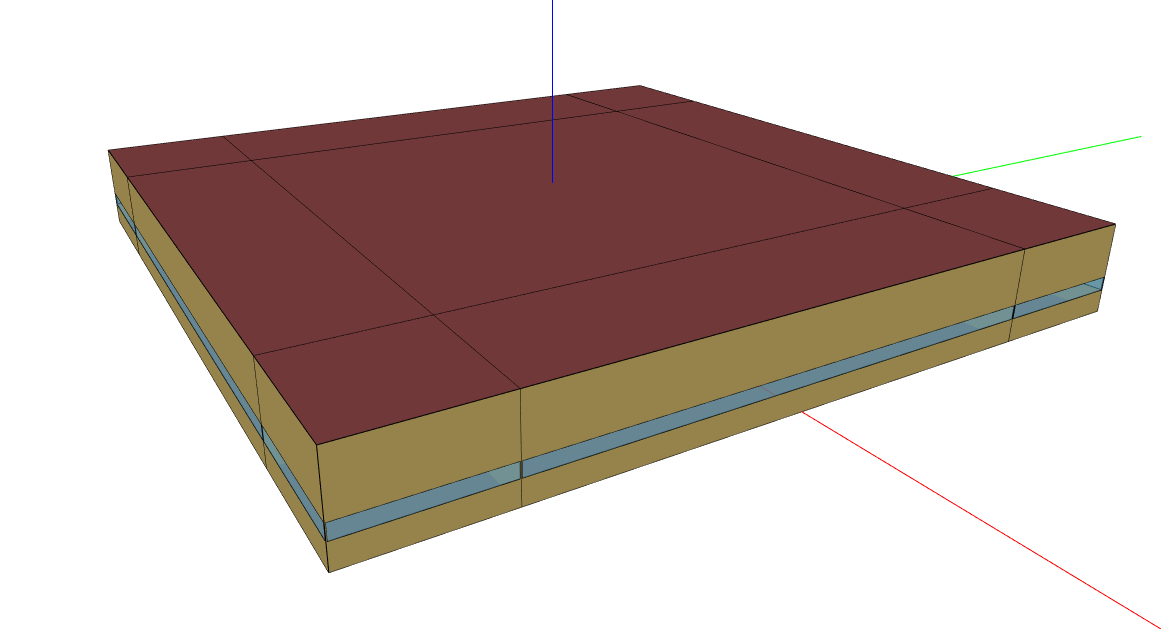
\includegraphics[width=0.7\textwidth]{figures/small_office_geometry.PNG}
    \caption[Example building geometry for a small office]{Example building geometry for a small office.}
    \label{fig:geom_example}
\end{figure}

\vspace{40mm} %blank space
\begin{center}
 (Intentionally blank)   
\end{center}


\pagebreak

\subsection{Area}
Building floor area is assigned to each model through the sampling process. Probability distributions were generated using CoStar \citep{costar} for most building types. HSIP \citep{hsip} was used for schools and hospitals, as neither are well represented in CoStar.

Figure~\ref{fig:area_dist} shows the breakdown of each building type in the national building stock by building size category (referred to as ``rentable area'').  Notice that the categories are presented as ranges.  At this time, ComStock uses the area in the middle of the range, with the exception of "\_1000" and "over\_1mil," which use 1000 square feet and 1 million square feet, respectively.  This method could be improved by adding variability to the building areas by selecting a variety of areas within the range.

\begin{figure}[H]
    \centering 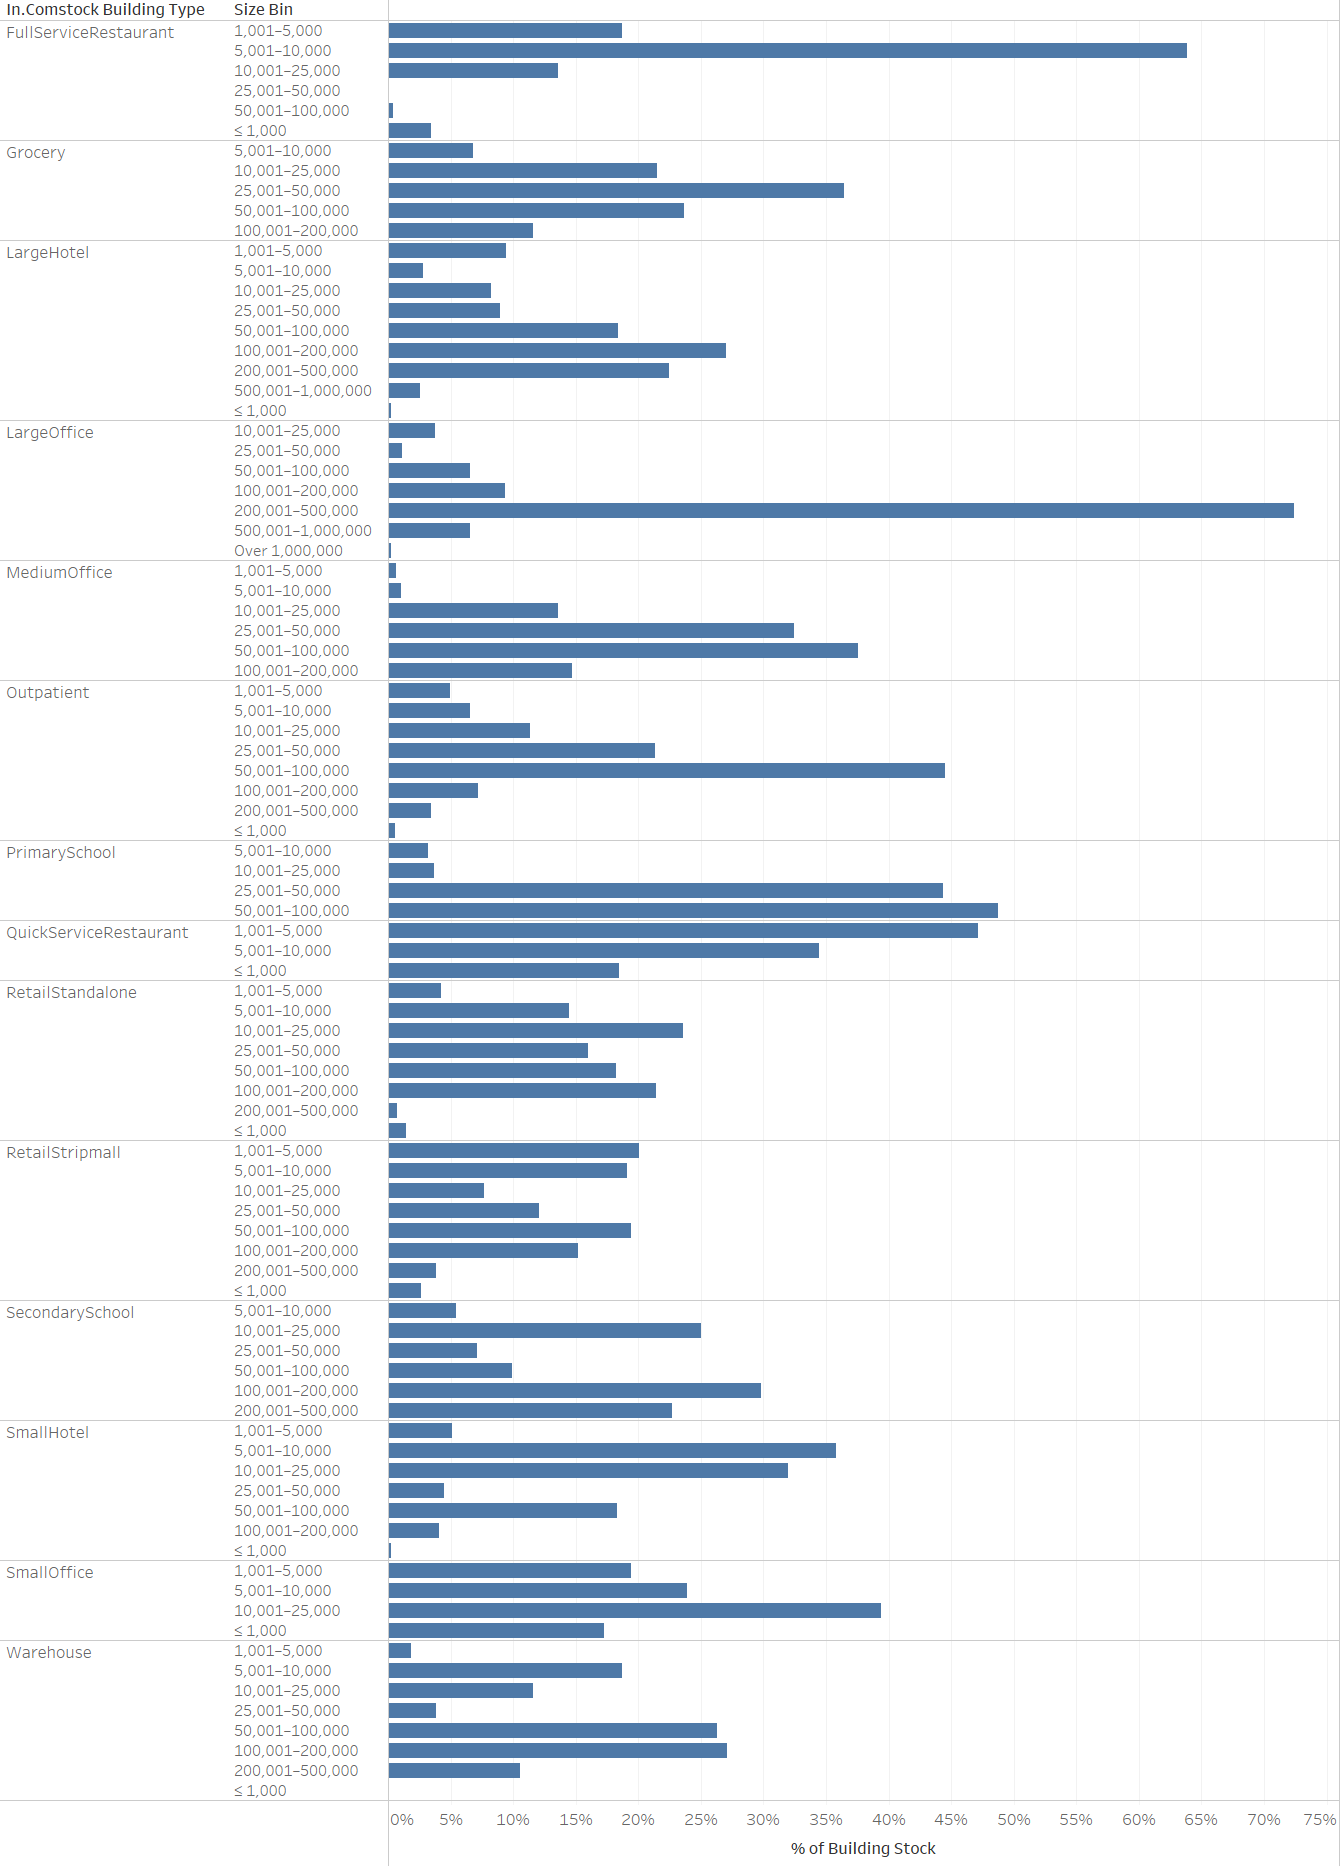
\includegraphics[width=1.0\textwidth]{figures/area_dist.png}
    \caption[Distribution of rentable area by building type]{Distribution of rentable area by building type. The x-axis represents rentable area (square feet), and the y-axis represents the fraction of the building stock.}
    \label{fig:area_dist}
\end{figure}

\pagebreak

\subsection{Building Shape}
Building shape is an intermediate characteristic assigned to the model during the sampling process. It is not a direct input to the model, as ComStock assumes a rectangular footprint for all buildings. Its function is as a dependency for aspect ratio (see next section \ref{subsec_aspect_ratio}). Probability distributions for building shape were generated from 2012 CBECS data, based on building type \citep{eia2012cbecs}. CBECS uses numbers to represent many of the answers to survey questions, and ComStock adopted these numbers to represent building shapes. 

Figure~\ref{fig:shape_dist} shows the breakdown of the national building stock by building shape and type. 

\begin{figure}[H]
    \centering 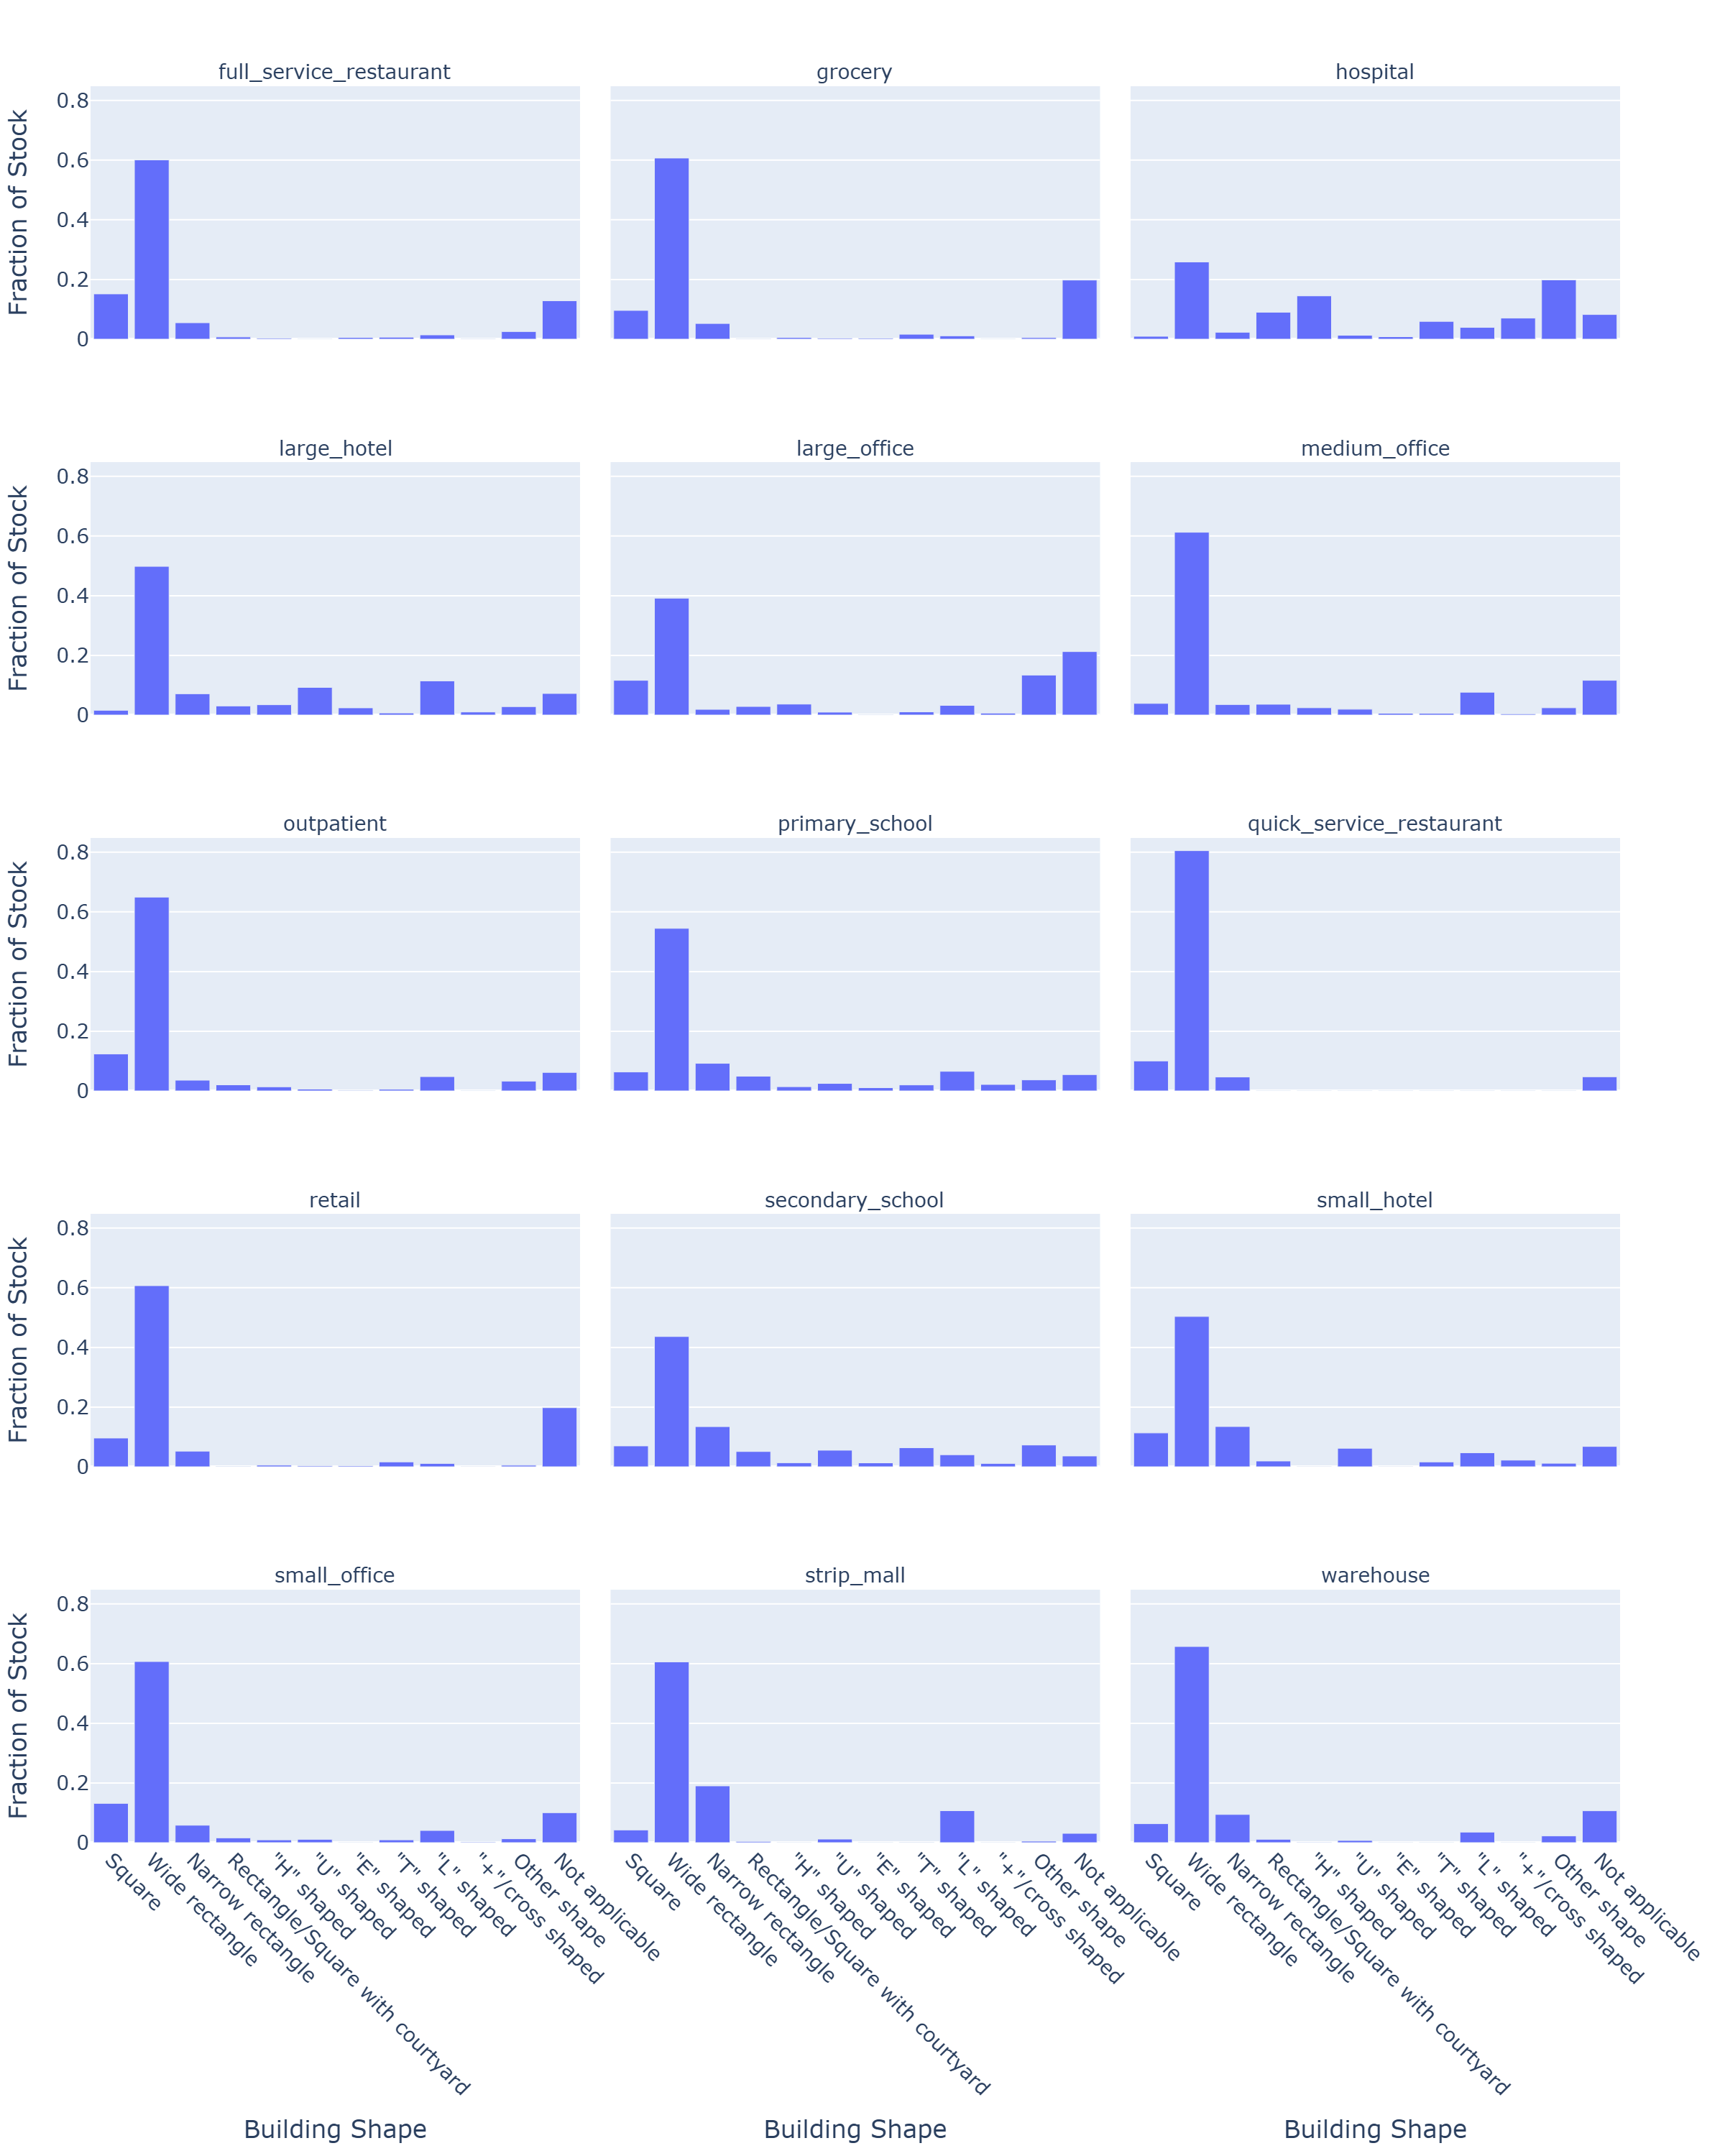
\includegraphics[width=1.0\textwidth]{figures/shape.png}
    \caption[Distribution of building shape by building type.]{Distribution of building shape by building type. The x-axis represents the building shape, and the y-axis represents the fraction of the building stock.}
    \label{fig:shape_dist}
\end{figure}

\pagebreak

\subsection{Aspect Ratio} \label{subsec_aspect_ratio}
Aspect ratio is defined as the overall length in the east–west direction divided by the overall length in the north–south direction. It is assigned to the building models during the sampling process. Probability distributions based on building shape were generated from 2012 CBECS data \citep{eia2012cbecs}.

Figure~\ref{fig:aspect_ratio_dist} shows the breakdown of the national building stock by aspect ratio. The aspect ratios are integers from one to six, which represent a building's north-south:east-west ratio.

\begin{figure}[H]
    \centering 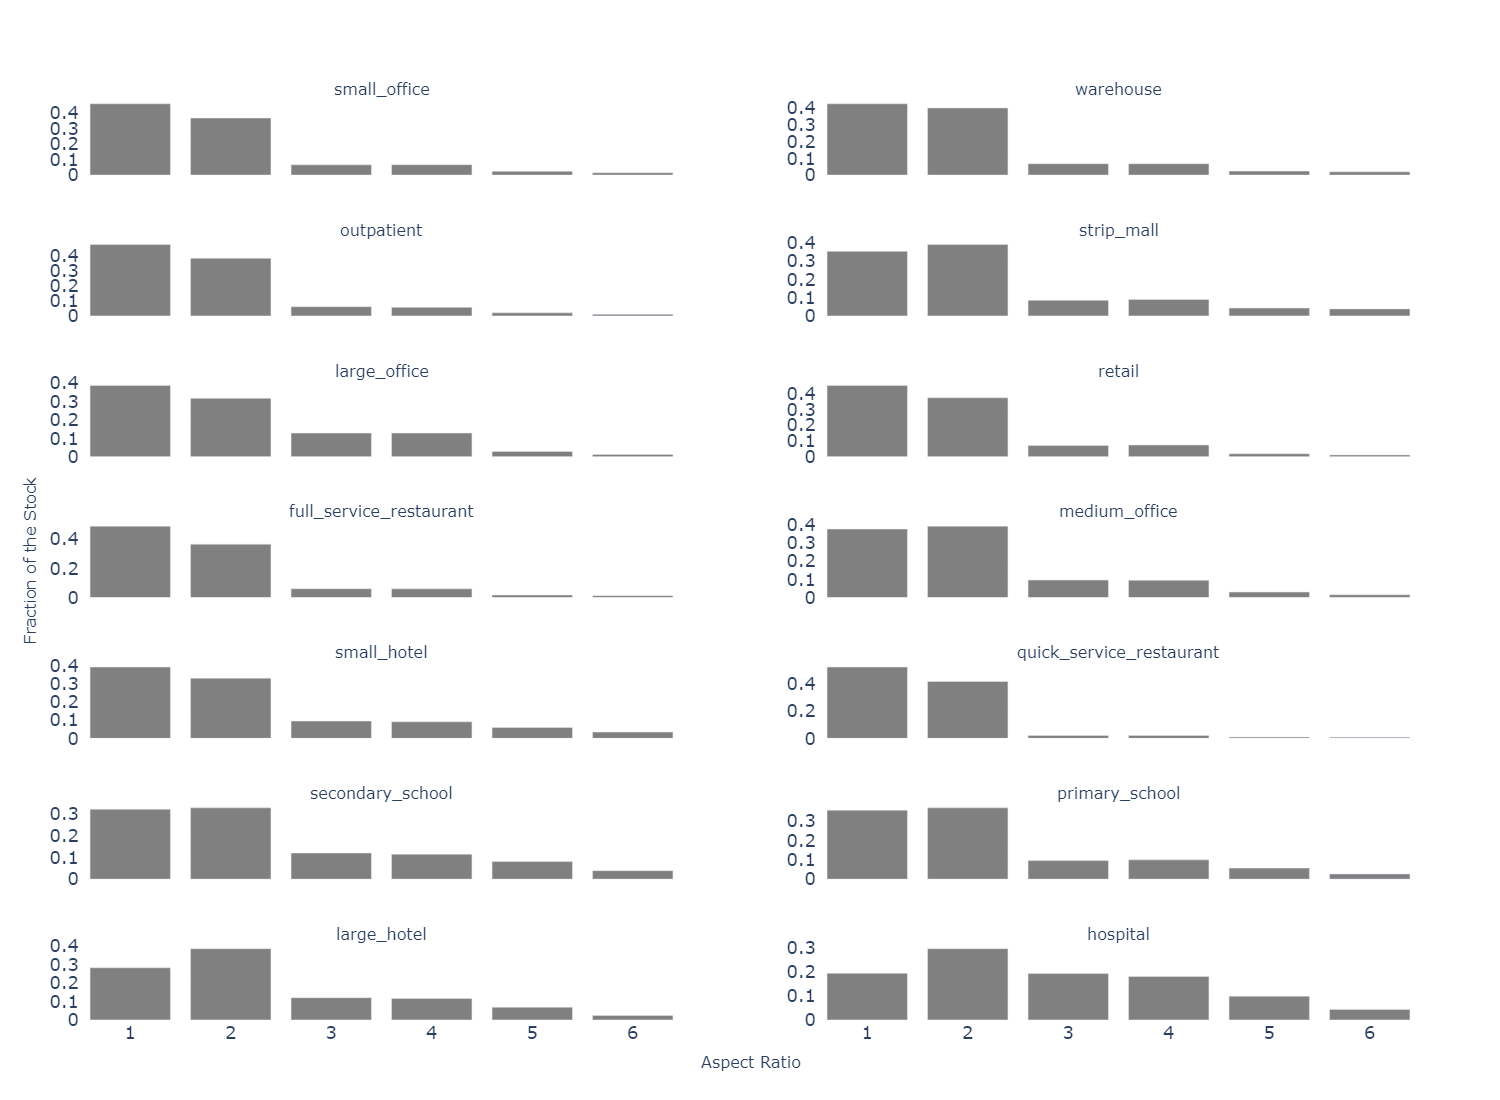
\includegraphics[width=1.0\textwidth]{figures/aspect_ratio.png}
    \caption[Distribution of aspect ratio by building type]{Distribution of aspect ratio by building type. The x-axis represents the aspect ratio (an integer from 1--6), and the y-axis represents the fraction of the building stock.}
    \label{fig:aspect_ratio_dist}
\end{figure}

\pagebreak

\subsection{Rotation}
Rotation defines the orientation of the building relative to the cardinal directions. In ComStock, there are eight rotation options, ranging from 0 to 315 degrees at 45-degree intervals. Ninety and 270 degrees correspond to a north-south length and east-west width (Figure~\ref{fig:rotation}). Rotations are evenly distributed throughout the building stock due to a lack of available data for more detailed distributions. This will be improved if new data becomes available.

\begin{figure}[H]
    \centering 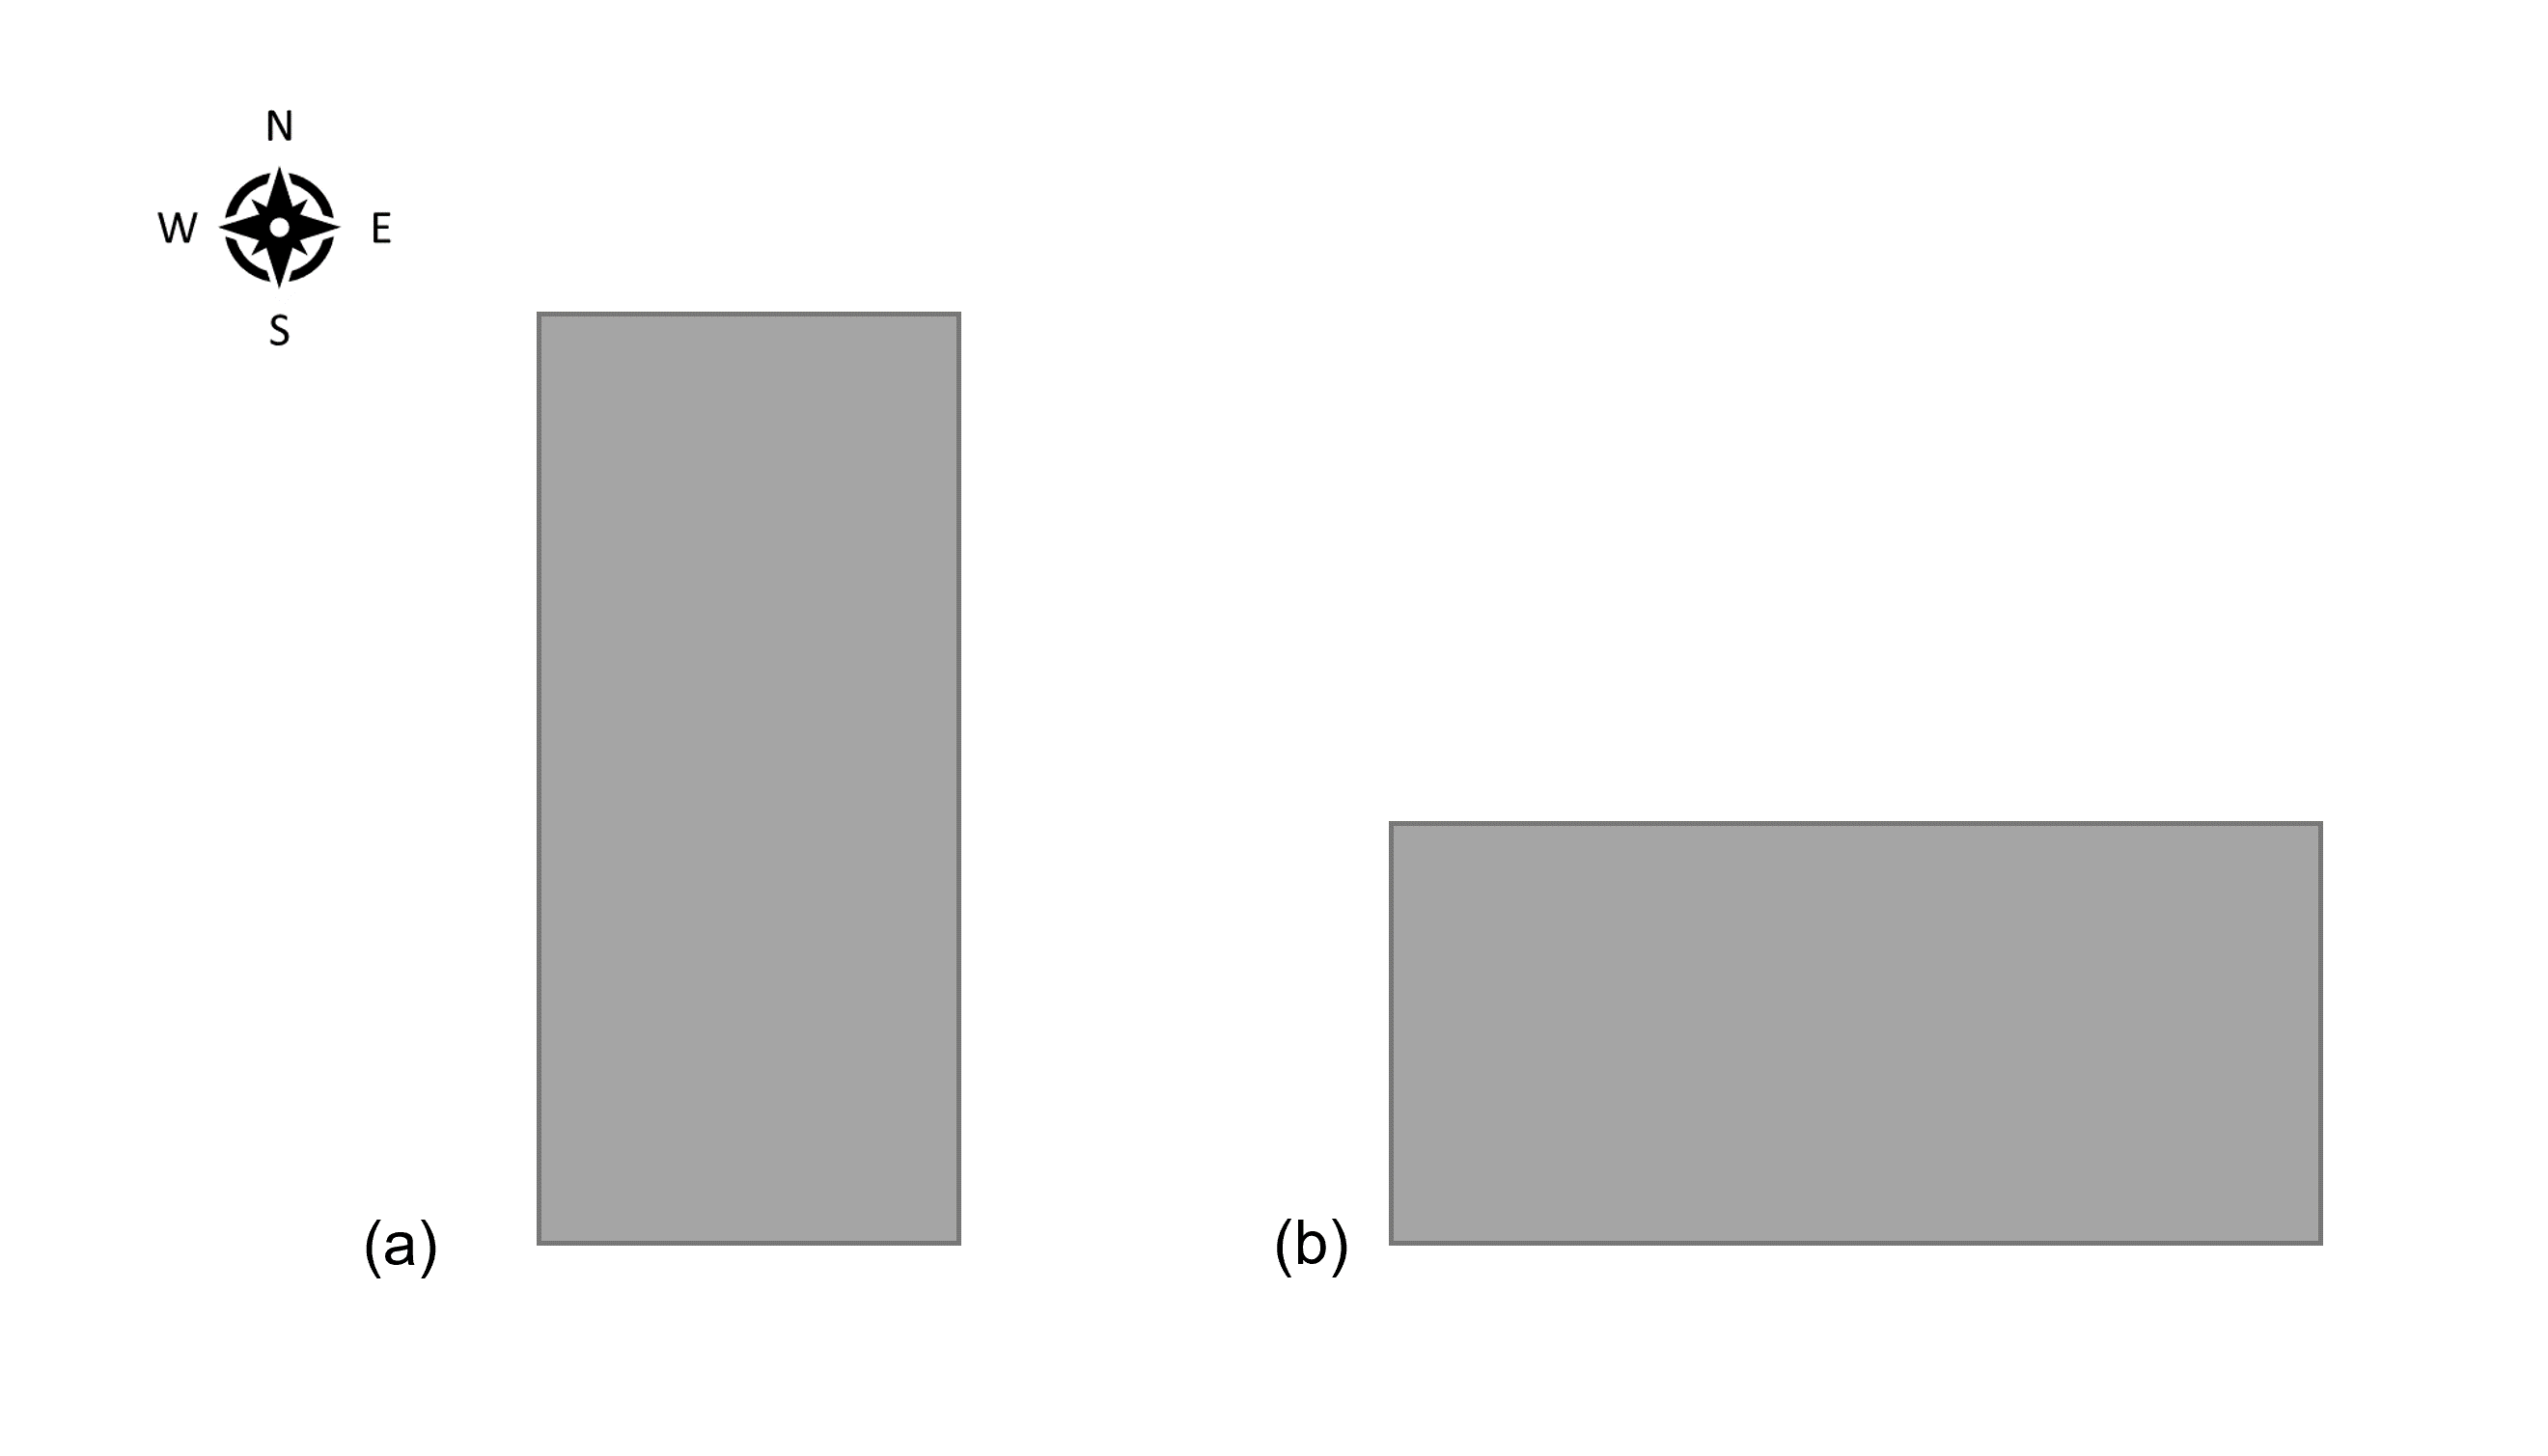
\includegraphics[width=0.7\textwidth]{figures/rotation_example.png}
    \caption[Building rotation]{Illustration of building rotation. (a) Buildings with either 90 or 270 degree rotation have a north-south length. (b) Buildings with either 0 or 180 degree rotation have an east-west length.}
    \label{fig:rotation}
\end{figure}

\subsection{Floor Height}
Floor height is represented in the models as floor-to-floor height. ComStock uses the floor-to-floor heights found in the DOE prototype buildings, which were established using expert opinion \citep{deru_2011}. These floor-to-floor heights are summarized in Table~\ref{tab:floor_height}.

\begin{table}[h]
\small
\centering
\caption[Floor-to-Floor Heights]{Floor-to-Floor Heights by Building Type}
\label{tab:floor_height}
\small
\begin{tabular}{|c|c|}
\hline
\textbf{Building Type}   & \textbf{Floor-to-Floor Height (feet)} \\ \hline
Full Service Restaurant  & 10                                    \\ \hline
Hospital                 & 14                                    \\ \hline
Large Hotel              & Ground: 13; Upper: 10                 \\ \hline
Large Office             & 13                                    \\ \hline
Medium Office            & 13                                    \\ \hline
Outpatient               & 10                                    \\ \hline
Primary School           & 13                                    \\ \hline
Quick Service Restaurant & 10                                    \\ \hline
Retail                   & 20                                    \\ \hline
Secondary School         & 13                                    \\ \hline
Small Hotel              & Ground: 11; Upper: 9                  \\ \hline
Small Office             & 10                                    \\ \hline
Strip Mall               & 17                                    \\ \hline
Warehouse                & 28                                    \\ \hline
\end{tabular}
\end{table}

\pagebreak

\subsection{Number of Floors}
ComStock assigns a number of floors to each model during the sampling process to create a distribution of building heights in the stock. This value represents the number of aboveground floors for a given model. No buildings in ComStock have belowground stories.

 For most of the building types, we generated probability distributions based on county and building type using CoStar \citep{costar}. We used HSIP \citep{hsip} for schools and hospitals, as neither are well-represented in CoStar.
 
 Figure~\ref{fig:nfloors_dist} shows the breakdown of the national building stock by number of floors and building type.

\begin{figure}[H]
    \centering 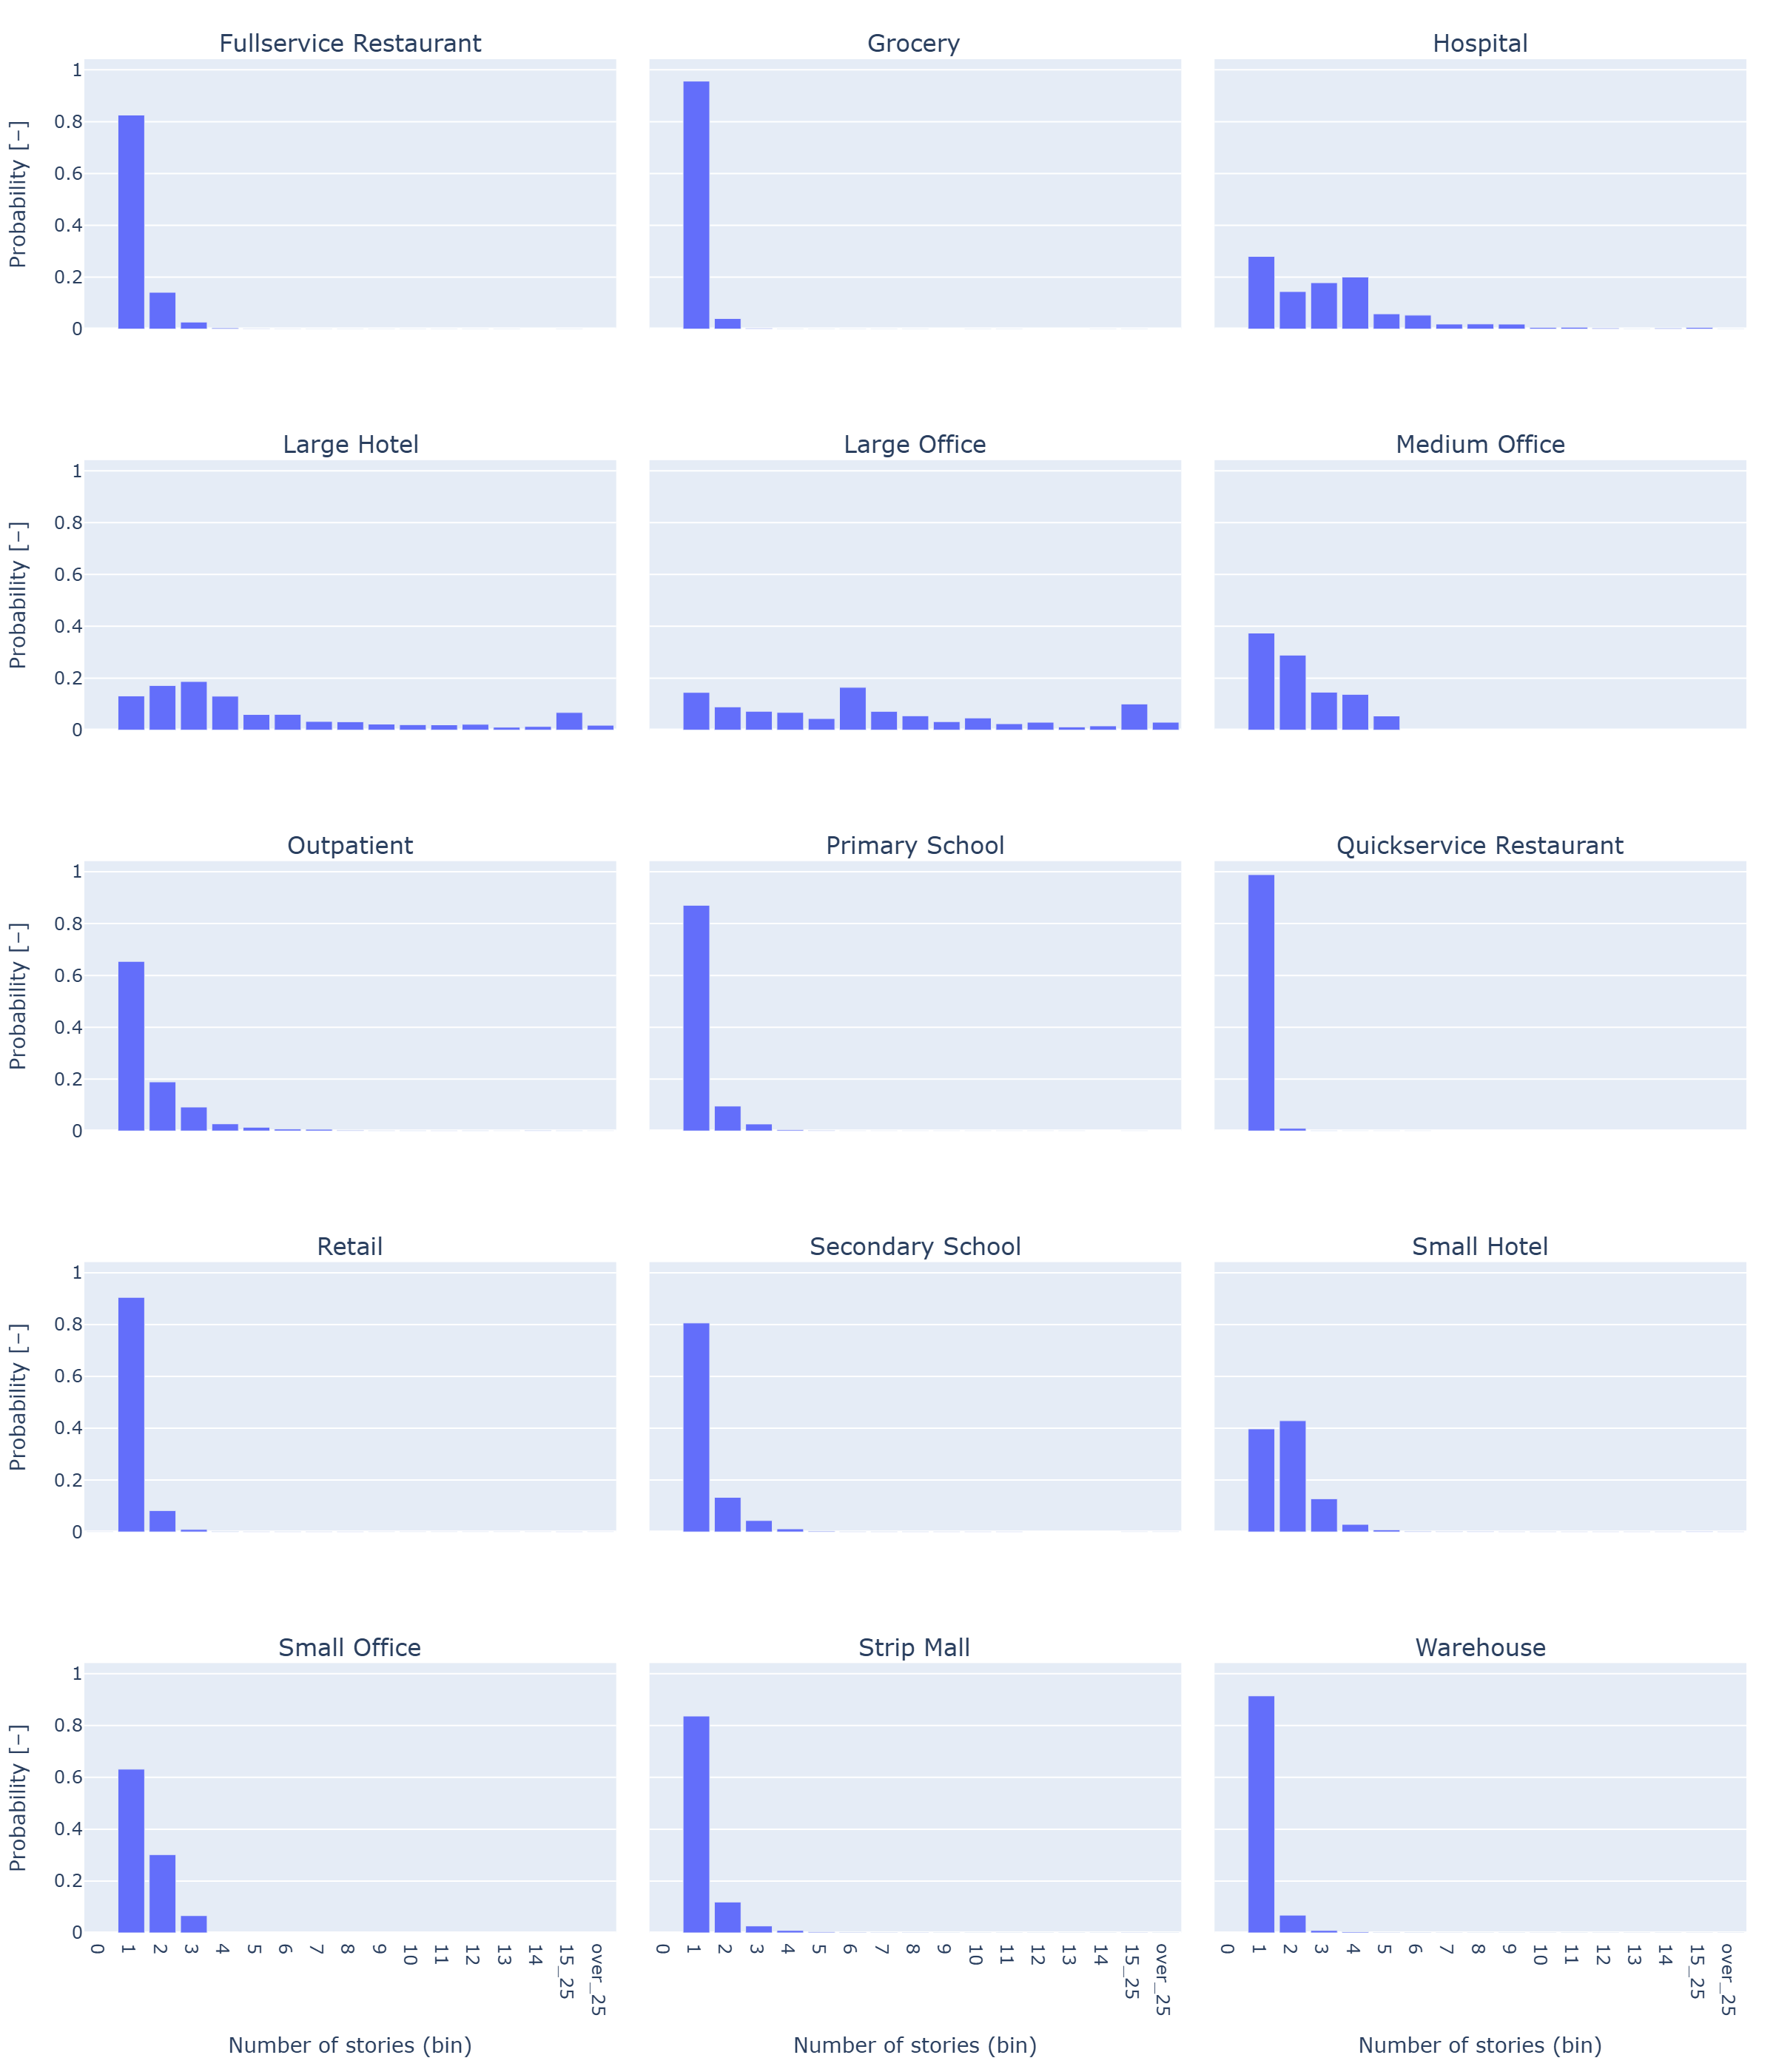
\includegraphics[width=1.0\textwidth]{figures/nfloors.png}
    \caption[Distribution of number of aboveground  floors by building type]{Distribution of number of aboveground  floors by building type. The x-axis represents the number of floors, and the y-axis represents the fraction of the building stock.}
    \label{fig:nfloors_dist}
\end{figure}

\pagebreak

\subsection{Window-to-Wall Ratio (WWR)}
The ComStock window-to-wall ratio (WWR) assumptions were created as part of the EULP project. WWR is defined as the fraction of abovegrade wall area that is covered by fenestration. Previously, ComStock used the WWR from the DOE prototype building models. Although each building type had a different WWR, there was no variability within each building type, which is not representative of the building stock. To address this issue, we referenced the NFRC Commercial Fenestration Market Study conducted by Guidehouse \citep{guidehouse_nfrc_window_report}. The study characterized the national commercial window stock through data collection and analysis. Six primary data sources representing all regions of the United States were used in the study---a 2020 Guidehouse survey, NEEA CBSA, DOE Code Study, CAEUS, CBECS, and RECS (multifamily). A variety of window properties were collected, including WWR, number of panes, frame material, glazing type, low-emissivity coating, gas fill, and many others. In total, the database contained approximately 16,000 samples, each with an appropriate weighting factor based on the coverage, completeness, and fidelity of each data source. We incorporated the WWR results from this study into the ComStock model, and we may incorporate other fields in the future to further refine our window modeling methodology.

From the Guidehouse data, we developed a WWR distribution for each combination of building type, floor area, and vintage. We first analyzed the WWRs separately by building type, floor area, geographic location, and vintage to determine which filters were appropriate to use for the final distributions. Geographic location did not have a significant impact on WWR, so it was left out of the final distributions. As can be seen in Figures~\ref{fig:wwr_by_rentable_area} and~\ref{fig:wwr_by_building_vintage}, there is a noticeable change in the WWR of buildings built after 2014, indicating that new buildings are trending toward larger windows. Similarly, there is a distinct trend in the WWR as a function of floor area; larger buildings tend to have more windows. Whereas the previous methodology only varied WWR by building type, these new distributions introduce more WWR variability by considering vintage and floor area.

The WWR distributions for all buildings before and after incorporating the NFRC data are shown in Figure \ref{fig:wwr_before_after_all_buildings}. The distinct bins in the graph are a result of the way WWR is binned in the CBECS Show Card: 0\%--1\% WWR is binned to 0.0, 2\%--10\% to 0.06, 11\%--25\% to 0.18, 26\%--50\% to 0.38, 51\%--75\% to 0.63, and 76\%--100\% to 0.88. The final distributions do not change the stock total energy consumption significantly, but they do add realistic variability within building types. For example, previously, all large offices had the same WWR of 0.15, whereas using the new distributions, large office WWRs vary from 0.01 to 0.88.

    \begin{figure} [h]
    \centering 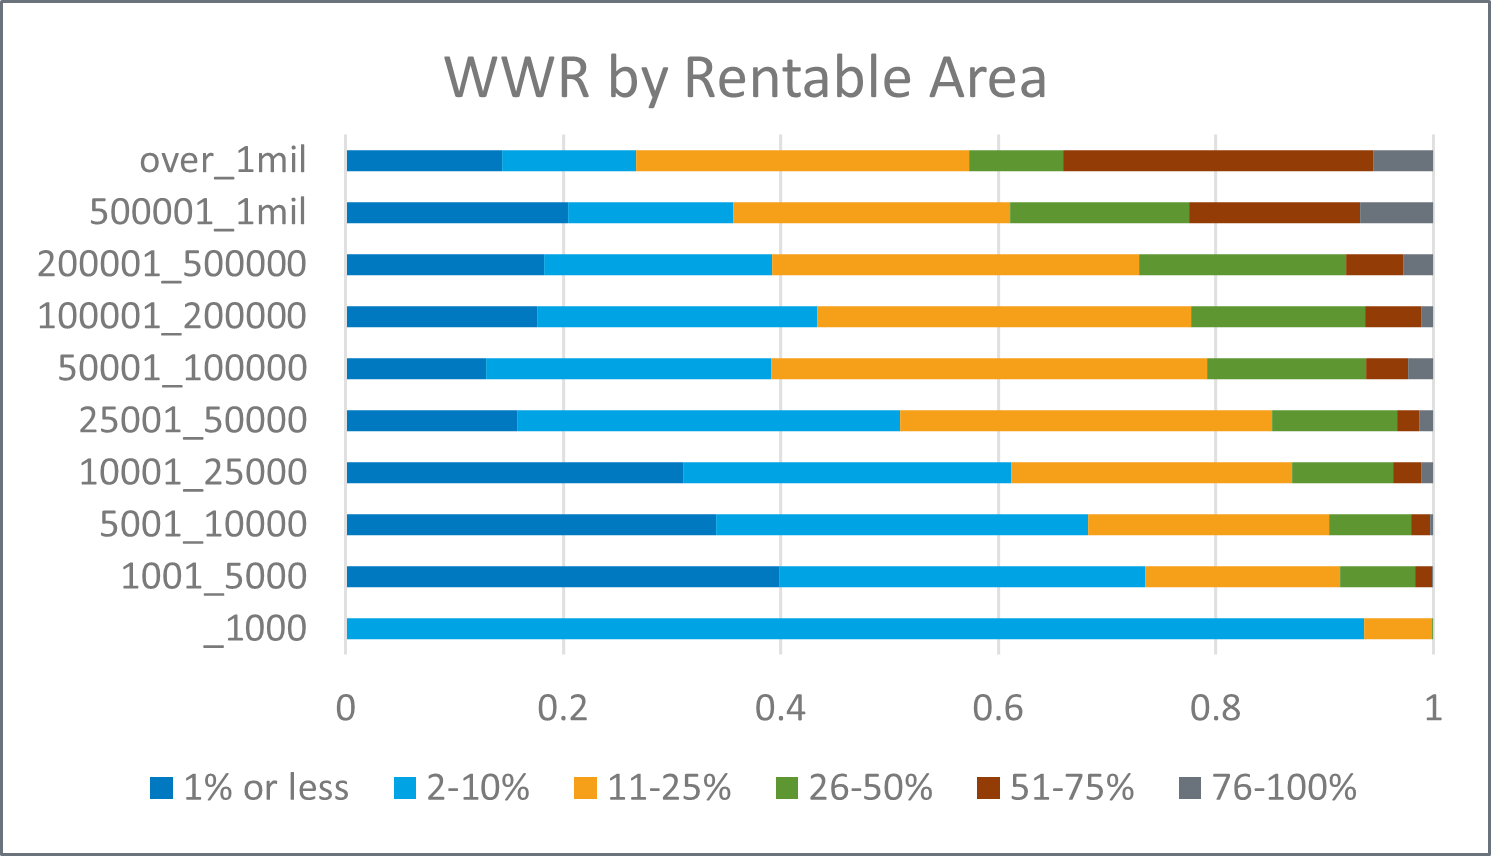
\includegraphics[width=\textwidth]{figures/wwr_by_rentable_area.png}
    \caption[Window-to-wall ratio by rentable floor area]{Window-to-wall ratio by rentable floor area.}
    \label{fig:wwr_by_rentable_area}
    \end{figure} 

\pagebreak

    \begin{figure} [h]
    \centering 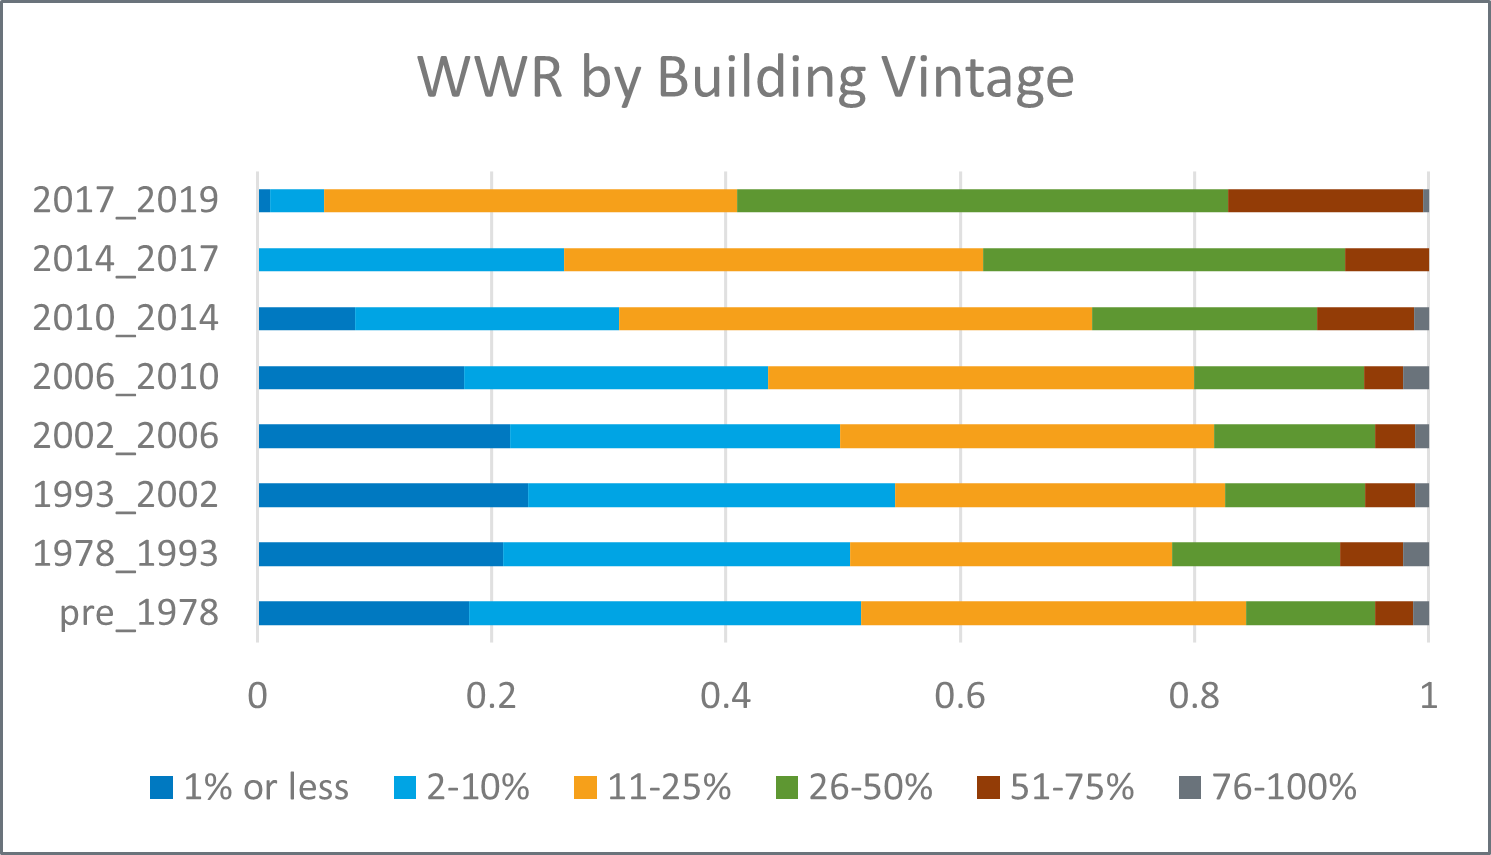
\includegraphics[width=\textwidth]{figures/wwr_by_building_vintage.png}
    \caption[Window-to-wall ratio by building vintage]{Window-to-wall ratio by building vintage.}
    \label{fig:wwr_by_building_vintage}
    \end{figure} 

    \begin{figure}[h!]
    \centering 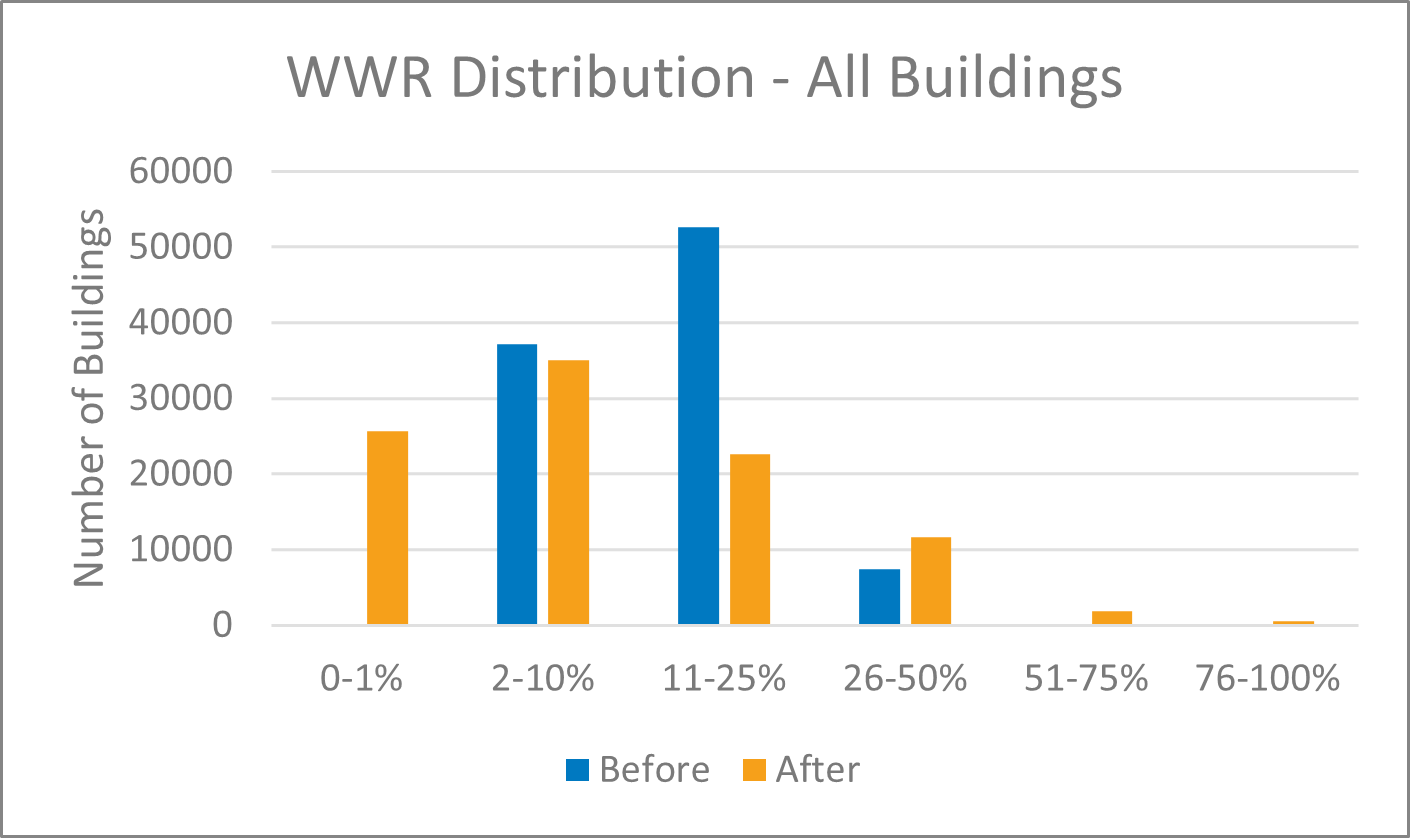
\includegraphics[width=\textwidth]{figures/wwr_before_after_all_buildings.png}
    \caption[Window-to-wall ratio distribution]{Window-to-wall ratio distribution in all building types before and after incorporating NFRC data.}
    \label{fig:wwr_before_after_all_buildings}
    \end{figure} 

\pagebreak

\subsection{Space Programming and Thermal Zoning}
As described above, all ComStock building models are a rectangular prism with a prescribed aspect ratio, floor area, etc. Within each building, there are one or more space types, as described in Section \ref{sec:space_type_ratios}. Space types are represented within the rectangular geometry as ``slices'' through the building that correspond to the floor area fractions of each space type. This is shown in Figure \ref{fig:geometry_by_space_type_and_zone}(a). In the cases of very small buildings, this can sometimes result in spaces which are unrealistically long and narrow for space types that make up only a small fraction of the building.

For larger buildings where the length and width are both greater than 37.5 feet, each space type is divided into core-and-perimeter thermal zones with a 15-foot depth (Figure \ref{fig:geometry_by_space_type_and_zone}(b)). Notice that the space types adjacent to the shorter ends of the building are each broken into six thermal zones, whereas the space types in the center of the building are each broken into three thermal zones. In multistory buildings, space types are often found on more than one floor, and in some cases, a floor will be a single space type. The downside to this thermal zoning approach is that thermal zones---and, as a follow-on, the HVAC systems that serve them---may be unrealistically small or large for certain geometry and building type combinations. These may later be modified to set a minimum and maximum size threshold for thermal zones.

\begin{figure}[hb!]
\centering 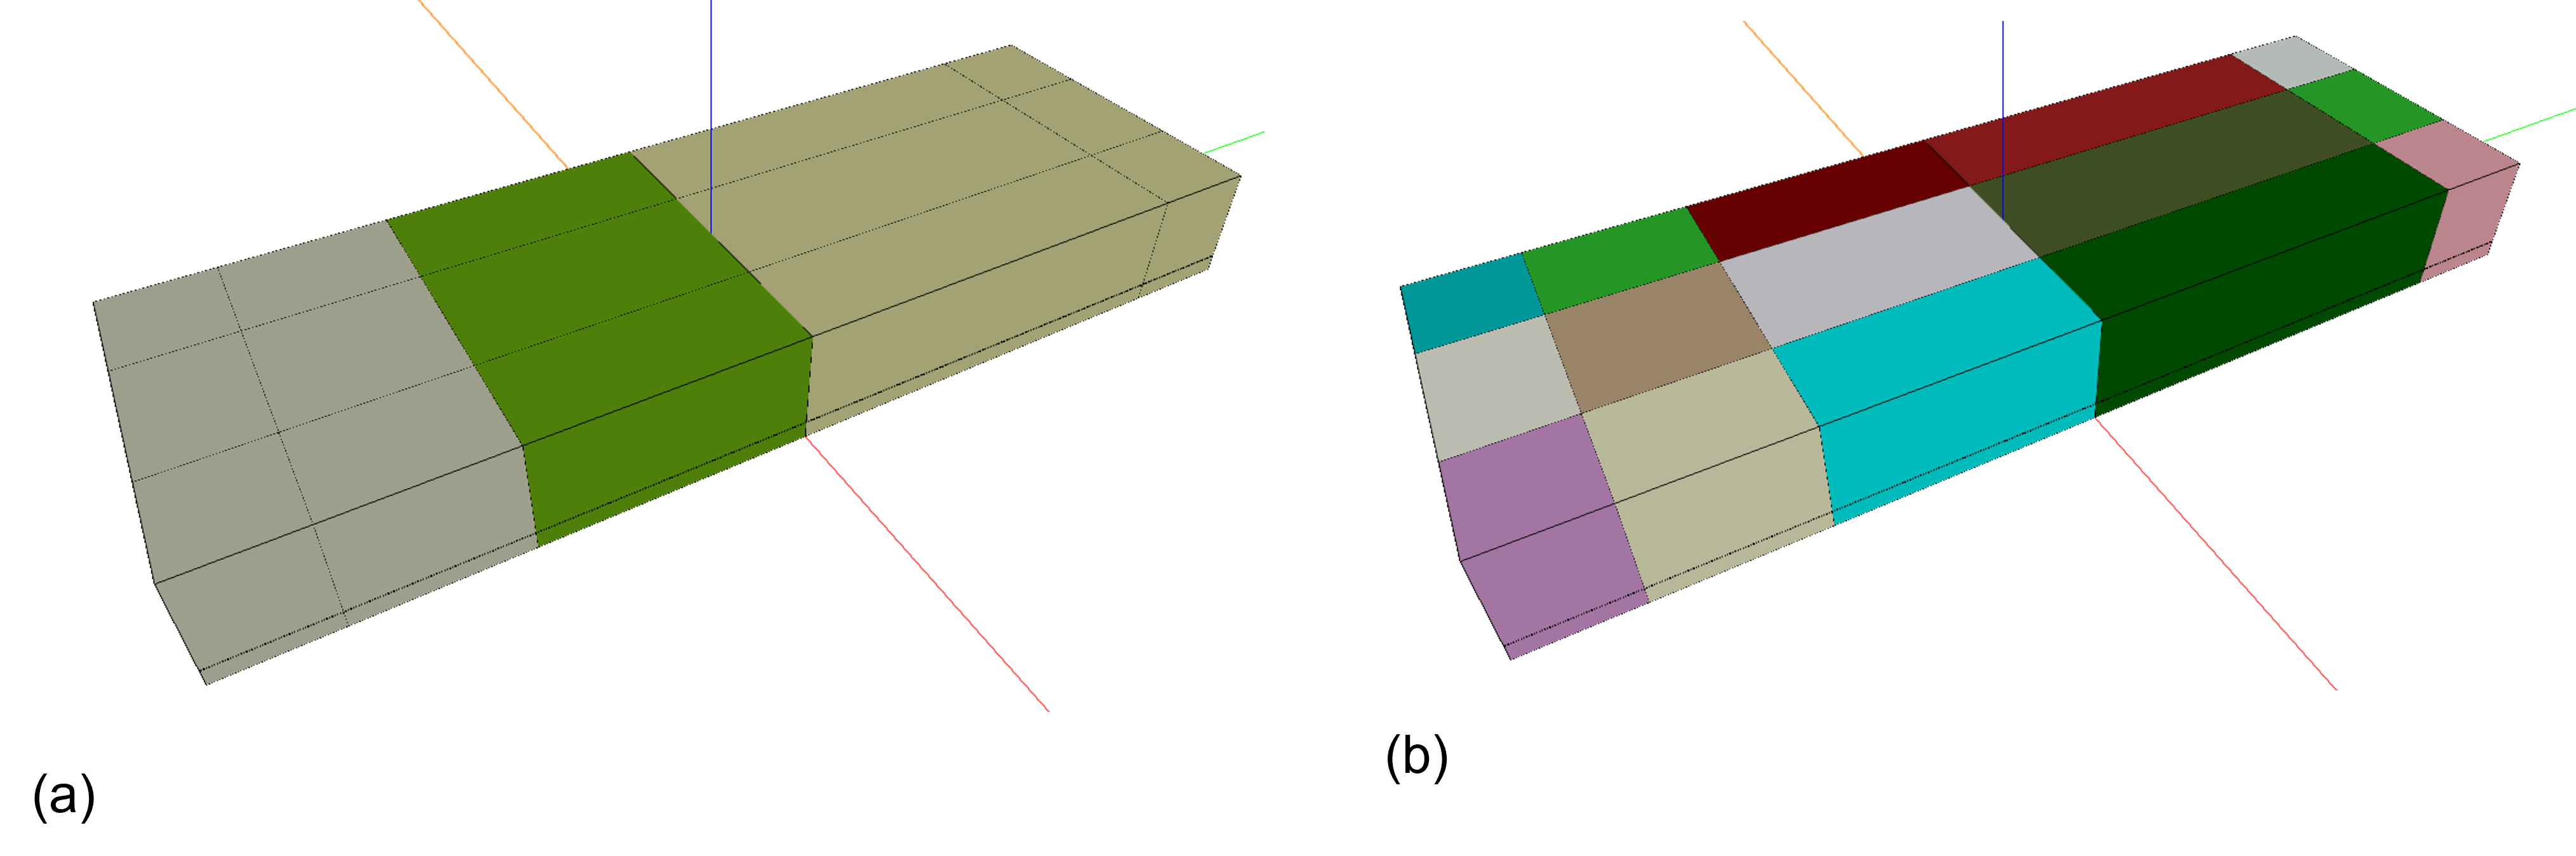
\includegraphics[width=1\textwidth]{figures/geometry_by_space_type_and_zone.png}
\caption[Example building geometry]{Example building geometry colored by (a) space type and (b) zone.}
\label{fig:geometry_by_space_type_and_zone}
\end{figure} 